% !TeX spellcheck = en_US
\documentclass[11pt, fleqn, titlepage]{article}
%\usepackage{siunitx}
\usepackage{texfiles/SpeedyGonzales}
\usepackage{texfiles/MediocreMike}
\newcommand{\so}[2]{{#1}\mathrm{e}{#2}}
% \geometry{top=1cm}
\usepackage{hyperref}
\usepackage{booktabs}
\hypersetup{
	colorlinks=true,
	linkcolor=blue,
	filecolor=magenta,      
	urlcolor=cyan,
}
\title{Phosphate in soil and the effect on barley production}
\author{Oskar Eiler Wiese Christensen s183917 \\ Anders Henriksen s183904 \\ \\ 02445 Project in Statistical Evaluation of Artificial Evaluation}
\date{\today \vspace{2.5cm} \section*{Abstract} \textit{The summary should contain a summary of the problem that  you are working with, which results you got, as well as main conclusions. \\ Don’t get into technical details. The summary should not be very long} \\ Lorem ipsum dolor sit amet, consectetur adipiscing elit, sed do eiusmod tempor incididunt ut labore et dolore magna aliqua. Gravida arcu ac tortor dignissim. Et netus et malesuada fames. Convallis posuere morbi leo urna molestie at elementum eu facilisis. Etiam erat velit scelerisque in dictum non. Mollis nunc sed id semper risus in hendrerit gravida. Cursus euismod quis viverra nibh cras pulvinar mattis nunc sed. Eu tincidunt tortor aliquam nulla. Duis convallis convallis tellus id interdum. Nunc lobortis mattis aliquam faucibus purus in massa tempor. Feugiat sed lectus vestibulum mattis ullamcorper. Malesuada proin libero nunc consequat interdum varius. Sed pulvinar proin gravida hendrerit lectus. Varius morbi enim nunc faucibus a. Ultricies leo integer malesuada nunc vel risus commodo viverra maecenas. Id aliquet lectus proin nibh nisl. Ullamcorper velit sed ullamcorper morbi tincidunt.}

\pagestyle{plain}
\fancyhf{}
\rfoot{Page \thepage{} of \pageref{LastPage}}

\graphicspath{{Billeder/}}

\begin{document}

\maketitle
%\thispagestyle{fancy}
%\tableofcontents

\section{Introduction}
\textit{Briefly introduce the background and setting of the problem, as well as the aim of the report. Furthermore, you could give a very short description of the analysis that will be applied.} \\ \\
The world is overpopulating. The population has grown exponentially over time while the surface of earth has naturally stayed constant. People have ever increasing problems with having enough space, both for living and agriculture. The latter will undoubtedly lead to huge agricultural problems, especially underproduction. One way to solve this issue could be to get a larger amount of cultivated land, which is not an effective long term solution as the population grows and the skirmish for proper households becomes ever tougher. The other option is to get more bang for your buck, or in other terms, getting a bigger yield from the same amount of land. There are many different ways of accomplishing this, but one would be to make sure to have large amounts of unbounded phosphate in the soil of the farmland, as this is a necessary nutrient for plant growth. Two possible measurements for this phosphorous amount are Olsen P and the newer, although more expensive, DGT measures. 

One natural and important question for farmers, which will be uncovered in this paper, is whether one measure is significantly different than the other and which measure is best, which will be determined by finding the measure with the lowest error on a non-linear fit to the data. Meanwhile, another interesting question for this paper is if the phosphorous amount even has a significant influence on the yield of the farms, which can be uncovered by a simple use of ANCOVA. The hypothesis prior to the carrying out of the experiments is that DGT should be a better measurement for determining the amount of bioavailable phosphorous is the soil, as this method is both more expensive and newer. Meanwhile, it is expected that the amount of bioavailable phosphorous should have a significant effect on the yield, as more plant nutrients should lead to bigger and stronger plants.

\section{Data}
\textit{Describe of the data you are analyzing. What kinds of data do you have, how were they collected (if applicable)? \\ Include a few good plots to highlight important features in data. You can put additional plots in the appendix.}\\
\noindent
The data consists of soils samples that were obtained from fields in Denmark and Norway respectively. Each field was divided into smaller subfields within the field, and barley was then sown on each of the subfields. On each of the subfields a soil sample was obtained and analyzed for bio-available phosphorus using two-methods, Olsen-P and DGT. Where Olsen-P is the traditional method and DGT is a newer and more expensive method. The data consists of four different variables; Location, yield, DGT measurement and Olsen-P measurement, as well as 36 different observations, 4 from each location except for location 9, where two of the yield measurements are missing. Location is a factor, while every other variable is continuous.
\\ \noindent 
Since both olsen-P and DGT is a measurement for the yield, it would be suspected that there is a correlation between both of the measurements. 
\begin{figure}[H]
	\centering
	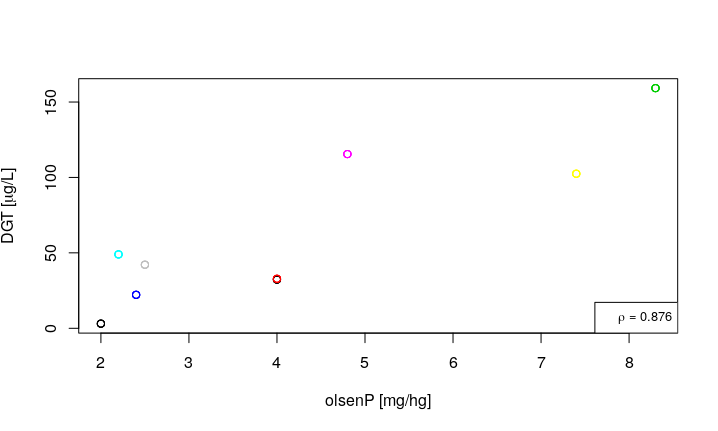
\includegraphics[width=0.7\linewidth]{billeder/dgtolsencor.png}
	\caption{Scatterplot of the DGT and olsenP measurement}
	\label{fig:dgtolsencor}
\end{figure}
\noindent It is seen from \ref{fig:dgtolsencor} that olsenP and DGT are indeed correlated. Hence, they both describe the same thing, but since the correlation is not equal to one the two measurements techniques do differ, which will be investigated in this project. To get an understanding of how yield is expressed in terms of DGT and Olens P values, the yield over DGT and yield over Olsen P plots are shown below. 


\begin{figure}[H]
	\centering
	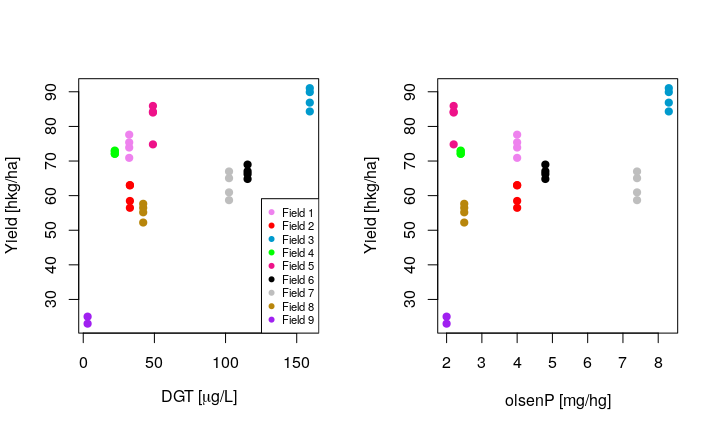
\includegraphics[width=0.7\linewidth]{billeder/measurementz}
	\caption{}
	\label{fig:measurementz}
\end{figure}

In \ref{fig:measurementz}, it is clear that low values of both DGT and Olsen P leads to a low yield, while somewhat higher values of DGT and Olsen P do not lead to much higher values of yield. This could suggest that the Michaelis-Menten model could be effective for fitting this data. This will be uncovered in the sections below.

\section{Methods}
\textit{Describe the methods you used and why you decided to use them. Also discuss the assumptions behind the methods. Do not go into detail with theory.}

\subsubsection*{Linear Regression}
In linear regression a linear model is fitted to the data. 

\[ y \approx a  \]

\subsubsection*{Non-linear Regression}
The second type of regression used to determine the measurement that best describes the yield is non-linear regression, which in this case was carried out using the Michaelis-Menten model, shown below.

\[y \approx \frac{\alpha \cdot x}{\beta \cdot x}, \quad x > 0 \]


\subsubsection*{Analysis of Covariance: ANCOVA}



\section{Results}
\textit{Present the results. \\ Tables and figures are good ways of illustrating results.}

For determining which measurement best describes the yield, the linear fits of the yield over DGT and yield over olsen P with accompanying $r^2$-values are shown below.

\begin{figure}[H]
	\centering
	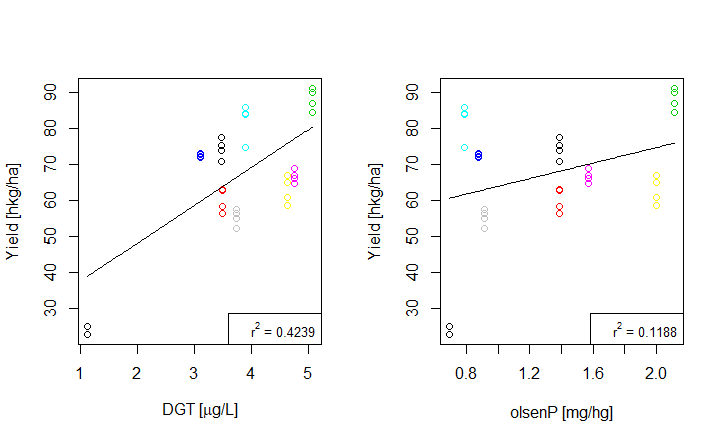
\includegraphics[width=0.7\linewidth]{billeder/Linearfit.png}
	\caption{}
	\label{fig:linearfit}
\end{figure}

\noindent The non-linear Michaelis-Menten fits of the yield over DGT and yield over olsen P with accompanying MSE-values are also shown below.

\begin{figure}[H]
	\centering
	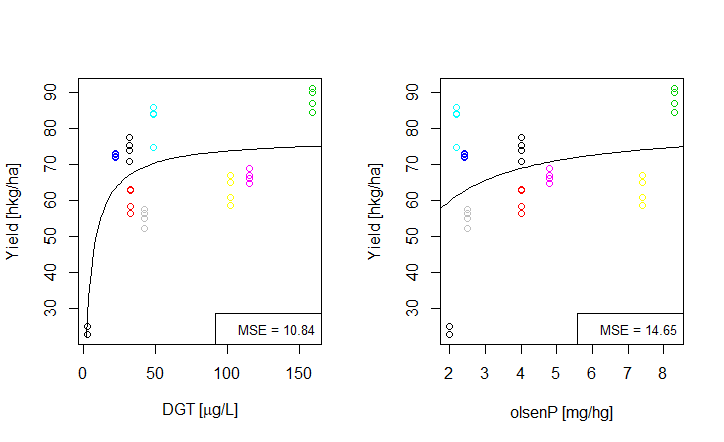
\includegraphics[width=0.7\linewidth]{billeder/non-linearfit.png}
	\caption{}
	\label{fig:non-linearfit}
\end{figure}

\noindent To investigate if the amount of bioavailable phosphorous has a significant influence on the yield, an ANCOVA is performed with yield as the response variable and Olsen P, DGT and location as the explanatory variables. This yields the following p-values.

\begin{table}[H]
	\centering
	\begin{tabular}{l r}
		\toprule
		Variable     & p-value                       \\ \midrule
		DGT          & $1.715 \cdot 10^{-10}$       \\ 
		Olsen P      & $7.621 \cdot 10^{-10}$         \\ 
		location     & $2.234 \cdot 10^{-16}$       \\ \bottomrule 
	\end{tabular}
\end{table}

\section{Discussion}
\textit{What do your results show? \\ Discuss your results. How reliable are they?}

\section{Conclusion}
\textit{What are your conclusions? The conclusion should be connected to the aim of the report in the introduction. \\ Highlight important results \\ If you have found interesting problems/aspects that you haven’t carried out, you can specify them here as ‘future work’.}

\section{Appendix}




\end{document}
